\subsection{Case01 - Drop}
\label{p4_ether_case01}
En este caso de uso se probará que es posible descartar todos los paquetes recibidos con un programa P4. Como tal, el programa P4 no es suficiente para probar esta funcionalidad, ya que requiere de una plataforma que sea capaz de soportar el lenguaje P4. Según se comentó en el capítulo de Análisis y Diseño (Cap. \ref{analisisPreimplementacion}), se hará uso de soft-switch llamado behavioral-model, \gls{bmv2} en adelante, para testear los programas P4 y de Mininet como escenario para recrear las topologías de Red. \\
\par

Antes de continuar con el caso de uso, se quiere remarcar un detalle importante. Continuamente se estará refiriendo al \gls{bmv2} como un ``switch", pero se debe entender que con el lenguaje P4 estamos definiendo el \textit{datapath} que tendrá la entidad que cargue con el programa P4, en este caso el  \gls{bmv2}. Por lo que, la denominación de switch puede no ser totalmente correcta, ya que depende del programa P4 que porte para comportarse como un switch. Nótese que el uso del término ``switch" deriva de la denominación de dispositivos programables en entornos SDN, que tradicionalmente se nombraron como ``switches" \\
\par

Debido a esto, el \gls{bmv2} puede actuar como un hub, un switch, un router o un firewall, etc. Dependerá de la funcionalidad implementada en el programa P4. Se aprovechará la interfaz implementada del \gls{bmv2} con Mininet, desarrollada desde la equipo de p4Lang, para conseguir integrar estos nodos en el escenario de red pudiendo así comprobar el funcionamiento del programa P4 desarrollado.\\
\par

\vspace{0.2cm}
\textbf{Compilación y puesta en marcha del escenario}\\
\par

Para la compilación del programa P4 se hará uso del compilador p4c. Este es el compilador de referencia para el lenguaje P4, es modular y permite escoger distintos \textit{targets} para llevar a cabo la compilación. El proceso de compilación de los programas P4 se lleva a cabo en dos etapas, una etapa de compilación de \textit{frontend} donde se genera un archivo \texttt{*.p4info}, el cual recoge todos los atributos necesarios del programa P4 en tiempo de ejecución ( identificadores de tablas, su estructura, \textit{actions}.. ), y una etapa de \textit{backend}, en la cual se hace uso del archivo generado \texttt{*.p4info} para generar los archivos necesarios para programar al \textit{target} en cuestión.\\
\par

% figura escenario
\begin{figure}[ht]
    \centering
    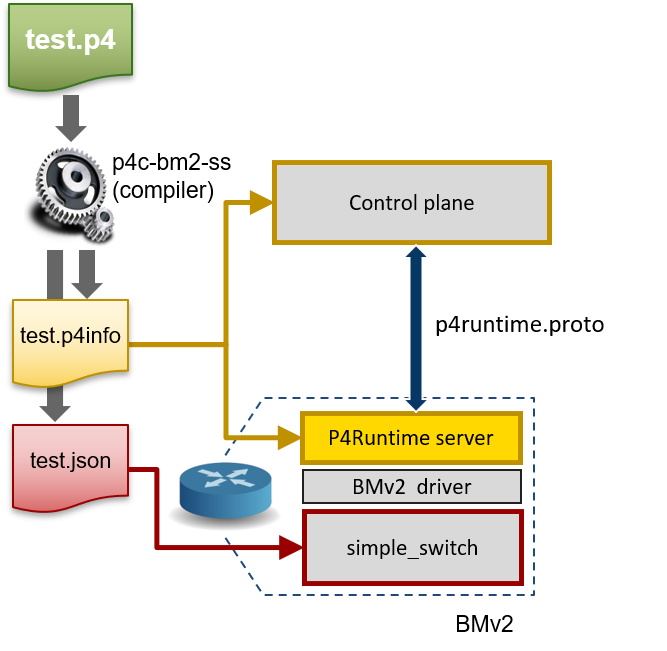
\includegraphics[width=5cm]{archivos/img/dev/p4/case01/compilation_bmv2.png}
    \caption{Proceso de compilación programa P4}
    \label{fig:case01_p4_ether_intro}
\end{figure}

Por ejemplo, el compilador de \textit{backend} que ataca al BMV2 genera un fichero \texttt{*.json}. Este fichero será suficiente para establecer todo el \textit{datapath} según lo programado en el programa P4. El target del compilador p4c que se utilizará es el \texttt{p4c-bm2-ss}, P4 simple\_switch - bmv2, el cual soporta la arquitectura \textbf{v1model}.\\
\par
Con la finalidad de poner en marcha del escenario, se ha dejado escrito un Makefile, el cual compilará el programa P4, generando los ficheros \texttt{*.p4info} y \texttt{*.json}. Acto seguido, se lanzará el script llamado \texttt{run\_exercise.py}, el cual levantará toda la topología descrita en el fichero \texttt{scenario/topology.json} con Mininet. Cada ``switch" de la topología tendrá implementada toda la lógica descrita en el programa P4 dentro de una instancia del \gls{bmv2}. A continuación, en la figura \ref{fig:case01_p4_ether_intro2} se puede ver una imagen resumen del levantamiento de un único ``switch".\\
\par
\vspace{0.5cm}
% figura escenario
\begin{figure}[ht]
    \centering
    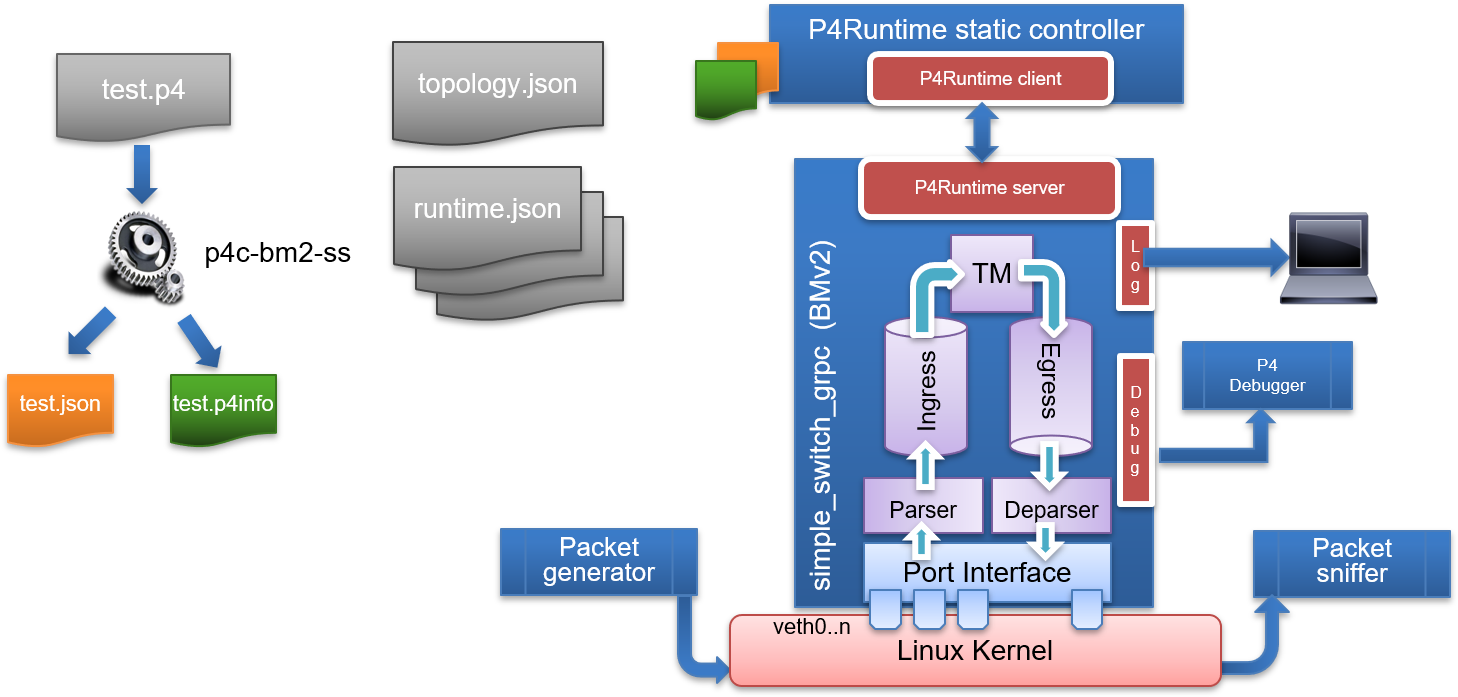
\includegraphics[width=15cm]{archivos/img/dev/p4/case01/setup.png}
    \caption{Proceso puesta en marcha de un switch BMv2 \cite{p42}}
    \label{fig:case01_p4_ether_intro2}
\end{figure}

\vspace{0.5cm}

Debido a que las personas que quieran replicar los casos de uso puede que no estén muy familiarizadas con todo este proceso de compilación y carga en los procesos de \gls{bmv2}, se ha dispuesto un de un Makefile para automatizar las tareas de compilación y carga de los programas, y también, para las tareas de limpieza del caso de uso una vez finalizada su demostración. Entonces, para proceder con la puesta en marcha del caso de uso, se deben seguir los pasos indicados en el bloque \ref{code:case01_p4_ether_load}.

\newpage

\begin{lstlisting}[language= bash, style=Consola, caption={Compilación programa P4 y puesta en marcha del escenario  - Case01},label=code:case01_p4_ether_load]
    # Entramos al directorio 
    cd TFG/src/use_cases/p4/case01

    # Hacemos uso del Makefile
    sudo make run
\end{lstlisting}
\vspace{0.5cm}

% figura escenario
\begin{figure}[ht]
    \centering
    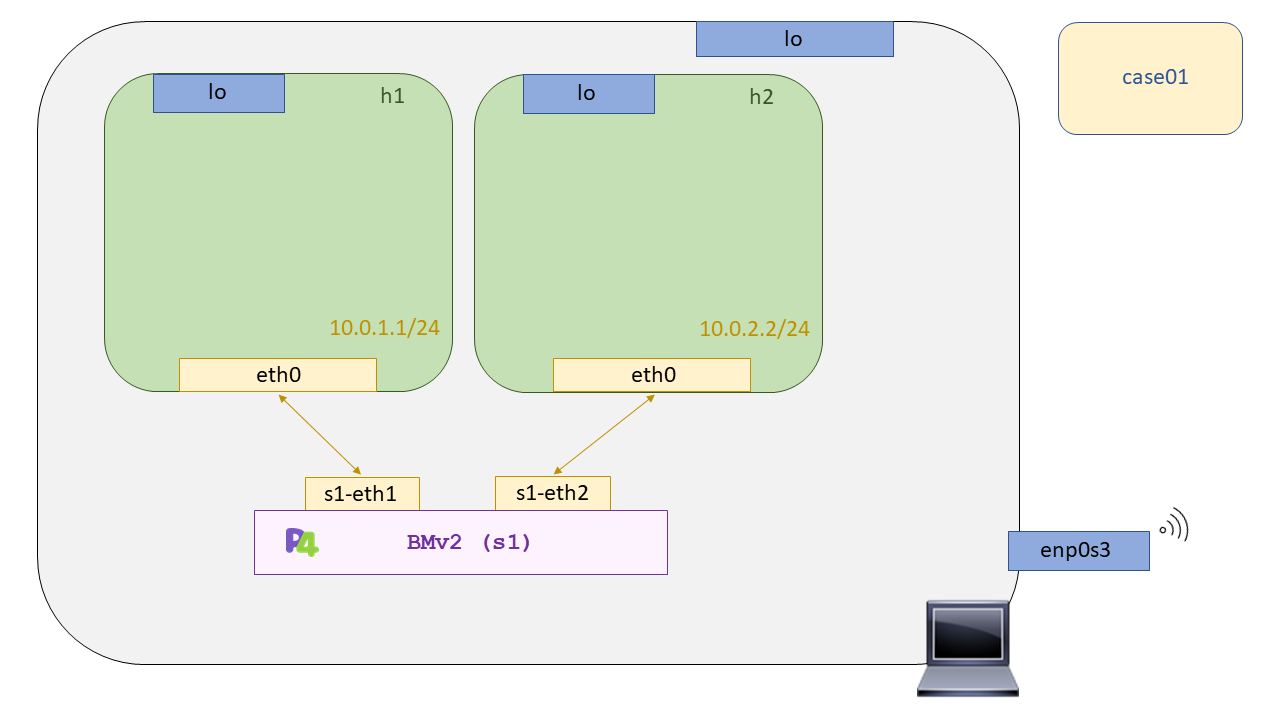
\includegraphics[width=16cm]{archivos/img/dev/p4/case01/scenario.png}
    \caption{Escenario del Case01 - P4}
    \label{fig:case01_p4_ether_scenario}
\end{figure}

Una vez se haya finalizado la comprobación del funcionamiento del caso de uso, se debe hacer uso de otro target (\textit{clean}) del Makefile para limpieza total del directorio.

\begin{lstlisting}[language= bash, style=Consola, caption={Limpieza del escenario P4 - Case01},label=code:case01_p4_ether_unload]
    # Hacemos uso del Makefile
    sudo make clean
\end{lstlisting}
\vspace{0.5cm}
Es importante señalar que este target limpiará tanto los ficheros auxiliares para la carga del programa P4 en el \gls{bmv2}, como los directorios de \texttt{pcaps}, \texttt{log}, y \texttt{build} generados en la puesta en marcha del escenario. Por lo que, si se desea conservar las capturas de las distintas interfaces de los distintos \gls{bmv2}, se deben copiar o limpiar del escenario a mano siguiendo las indicaciones del bloque \ref{code:case01_p4_ether_unload2}.

\begin{lstlisting}[language= bash, style=Consola, caption={Limpieza segura del escenario P4 - Case01},label=code:case01_p4_ether_unload2]
    # Limpiamos Mininet
    sudo mn -c
    
    # Limpiamos los directorios generados dinámicamente en la carga del escenario
    sudo rm -rf build logs
\end{lstlisting}


\vspace{0.5cm}
\textbf{Comprobación del funcionamiento}\\
\par

Una vez realizado el \texttt{make run} en este directorio, se tendrá levantada la topología descrita para este caso de uso, la cual se puede apreciar en la figura \ref{fig:case01_p4_ether_scenario}. La topología de este caso de uso se compondrá de una instancia del \gls{bmv2} (\texttt{s1}), y de dos host (\texttt{h1}, \texttt{h2}) que se conectarán al ``switch". Como ya se comentaba anteriormente, la topología puede encontrarse descrita bajo el directorio \texttt{scenario}, en un fichero JSON llamado \texttt{topology.json}. En este fichero también se describe la localización de los archivos que describen el plano de control de cada ``switch" de la topología. En todos los casos de uso, se ha respetado los nombres tipo utilizados por la organización de p4Lang, \texttt{sX-runtime.json}, donde X es el número que ocupa dicho switch en la topología de Mininet. Volviendo de nuevo a la comprobación del funcionamiento del caso de uso, se tendrá la CLI de Mininet abierta, por lo que se abrirá una terminal para el \texttt{host1} y otra para el \texttt{host2}.

\begin{lstlisting}[language= bash, style=Consola, caption={Comprobación de funcionamiento - Case01},label=code:case01_p4_ether_func]
    mininet>  xterm h1 h2
\end{lstlisting}
\vspace{0.5cm}

Ahora con ambas terminales abiertas, desde el \texttt{h2} se pondrá a escuchar por su interfaz. Se puede utilizar wireshark, o el sniffer que el lector crea conveniente. En este caso por simplicidad y no disponer de una interfaz gráfica, se utilizará tcpdump (\ref{tcpdump}).

% figura escenario
\begin{figure}[ht]
    \centering
    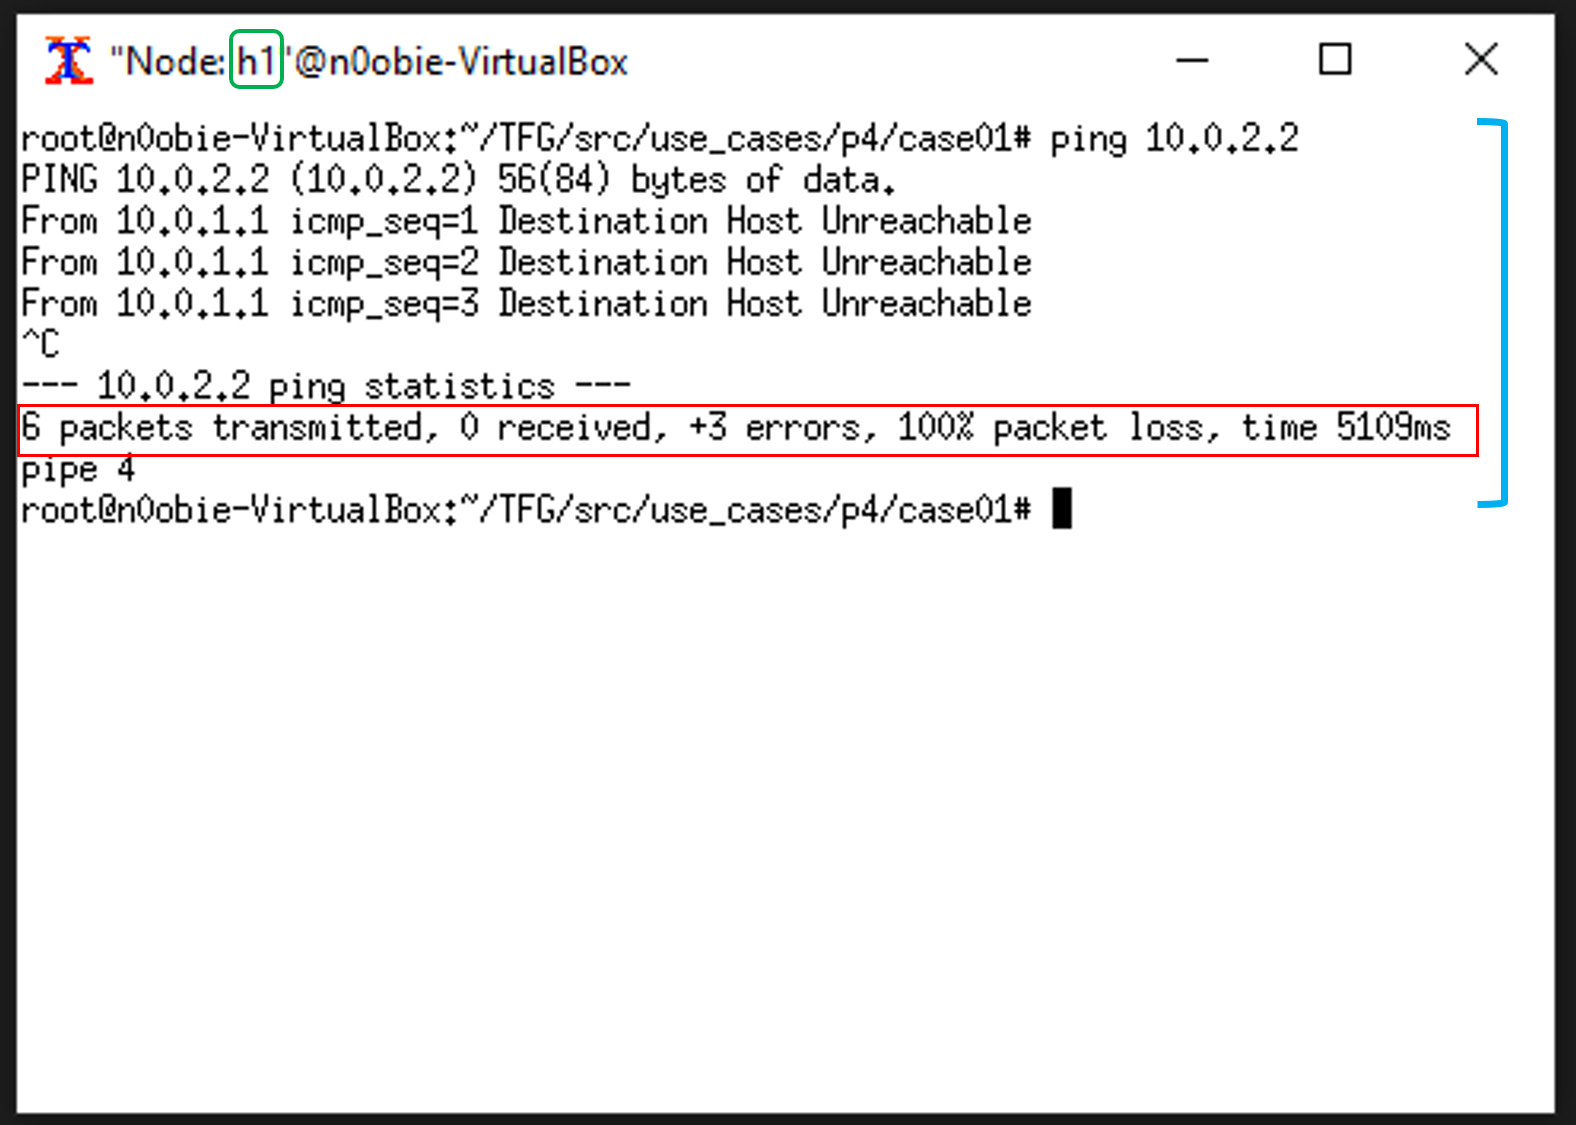
\includegraphics[width=9cm]{archivos/img/dev/p4/case01/demo_case01_1_edited.png}
    \caption{Comprobación de funcionamiento (Ping) del Case01 - P4}
    \label{fig:case01_p4_ether_func1}
\end{figure}
\newpage
\begin{figure}[ht]
    \centering
    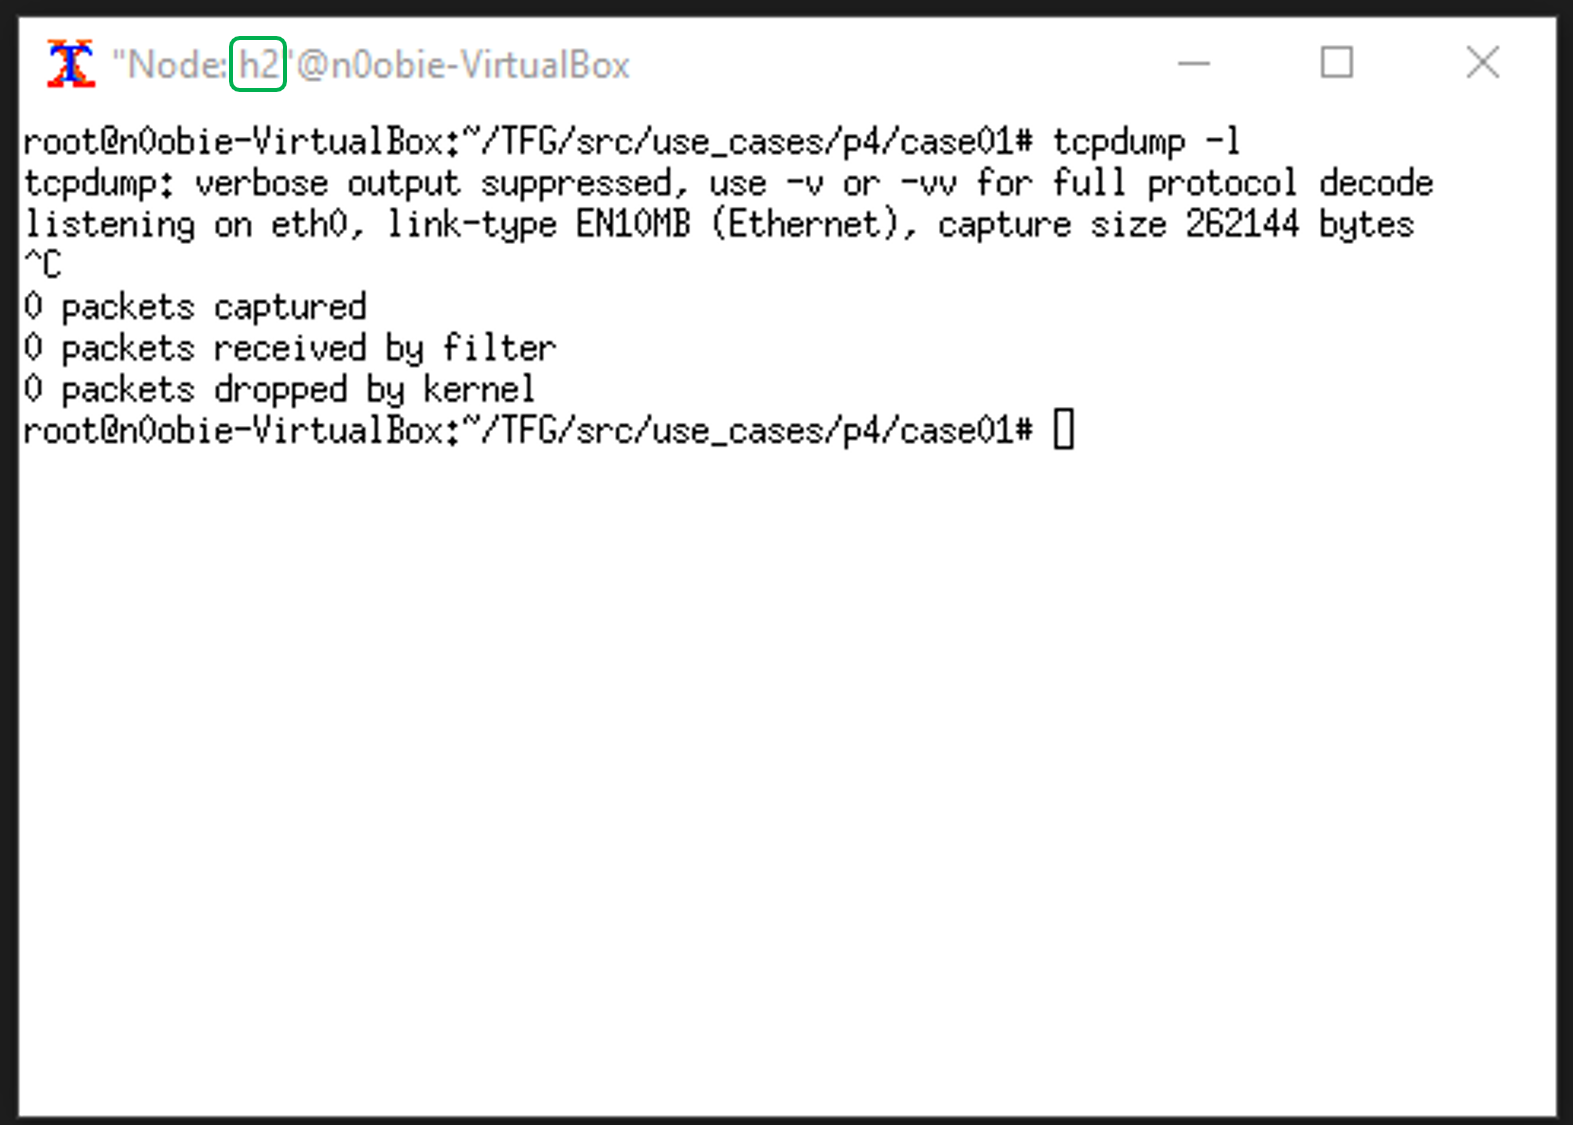
\includegraphics[width=11cm]{archivos/img/dev/p4/case01/demo_case01_2_edited.png}
    \caption{Comprobación de funcionamiento (Sniffer) del Case01 - P4}
    \label{fig:case01_p4_ether_func2}
\end{figure}


Una vez que se esté escuchando en la interfaz del \texttt{host2}, se hará ping \fcolorbox{black}{ProcessBlue}{\rule{0pt}{2.5pt}\rule{2.5pt}{0pt}}\hspace{1mm} desde el \texttt{host1} al \texttt{host2} y no se debería tener conectividad. Como se puede ver en las figuras \ref{fig:case01_p4_ether_func1} y \ref{fig:case01_p4_ether_func2}, el programa P4 desarrollado funciona correctamente. Para asegurarse de que realmente se está ejecutando el action para tirar paquetes se puede consultar los logs del \gls{bmv2}, los cuales generan un fichero de log por cada instancia target del simple switch que se haya levantado. \\
\par
Estos logs se encuentran en el directorio \texttt{logs}, y cada fichero de log pertenece a un único ``switch", llevando el mismo nombre que este en Mininet. En este caso, si se quisieran monitorizar los logs del \texttt{s1} bastaría con seguir las indicaciones del bloque \ref{code:case01_p4_ether_func2}.

\begin{lstlisting}[language= bash, style=Consola, caption={Comprobación de funcionamiento - Case01},label=code:case01_p4_ether_func2]
    # Entramos al directorio 
    cd TFG/src/use_cases/p4/case01

    # Monitorizamos los logs del Switch (s1) 
    tail -f logs/s1.log
\end{lstlisting}